%===========================================================
\subsection{Problem}
%===========================================================
\begin{frame}{Example Problem: Heat Equation}
  \begin{itemize}
  \item
    Demonstrate FEM using steady-state heat equation (omitting technical details)
    \begin{align*}
      \nabla^2 u &= 0 &\forall \;\;\tensor{x}&\in \Omega \\
      u &= \hat{u}(\tensor{x}) &\forall \;\;\tensor{x} &\in \partial \Omega_D \\
      \nabla u \cdot \tensor{n} &= g(\tensor{x}) &\forall \;\; \tensor{x} &\in \partial \Omega_N
    \end{align*}
  \item
    As written, this PDE applies point-wise throughout the domain $\implies$ ``Strong Form''
  \end{itemize}
\end{frame}


%===========================================================
\begin{frame}{Weak Form}

  \begin{itemize}
  \item
    For FEM, we transform the PDE to the ``weak form''
  \item
    Multiply by a ``test function'' $v$ that satisfies boundary conditions and 
    certain integrability requirements, then integrate by parts
    \begin{align*}
      \int_{\partial \Omega_N} v (\nabla u \cdot \tensor{n})\,\mathrm{d}A - 
      &\int_{\Omega} \nabla v \cdot \nabla u \dV = 0  \\
      &\forall\;\; v \in 
      \{\text{a set satisfying above requirements}\}
    \end{align*}
  \end{itemize}

\end{frame}


%===========================================================
\subsection{Spatial Discretization}
%===========================================================
\begin{frame}{Discretize Domain}

  \begin{columns}
    \begin{column}{.5\textwidth}
      \begin{itemize}
      \item
        Express integrals over whole domain as sum of integrals over elements
        \begin{align*}
          \int_\Omega \nabla v \cdot &\nabla u \dV = \\
          &\sum_e \int_{\Omega_e} \nabla v \cdot \nabla u \dV
        \end{align*}
      \end{itemize}
    \end{column}
    \begin{column}{.5\textwidth}
      \begin{figure}
        \centering
        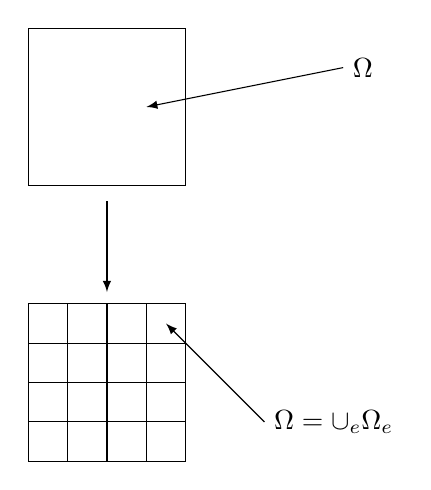
\begin{tikzpicture}[scale=2.0]
          %original box
          \draw (0,0) -- (1,0) -- (1,1) -- (0,1) -- (0,0);
          
          \draw[latex-] (.75, .5) -- (2,.75) node[right]{$\Omega$};
          
          % down arrow
          \draw[-latex] (0.5, -0.1) -- (0.5, -0.675);

          \draw (0,-1.75) -- (1,-1.75) -- (1,-0.75) -- (0,-0.75) -- (0,-1.75);
          \draw (0,-1.5) -- (1,-1.5);
          \draw (0,-1.25) -- (1,-1.25);
          \draw (0,-1) -- (1,-1);
          \draw (0.25,-0.75) -- (0.25,-1.75);
          \draw (0.5,-0.75) -- (0.5,-1.75);
          \draw (0.75,-0.75) -- (0.75,-1.75);
          \draw[latex-] (.875, -0.875) -- (1.5,-1.5) node[right]{$\Omega = \cup_e \Omega_e$};
        \end{tikzpicture}
      \end{figure}
    \end{column}
  \end{columns}

\end{frame}


%==============================================================
\begin{frame}{Change of integration bounds}

  \begin{columns}
    \begin{column}{0.5\textwidth}
      \begin{itemize}
      \item
        Generally, elements are not regular rectangles, so
        we change bounds of integration to an easier element
        shape to integrate over
      \item
        This easier shape is called the ``parent'' or ``canonical'' element
      \item
        For quadrilaterals, the canonical element is $\Omega_0 = [-1, 1] \times [-1, 1]$
      \end{itemize}
    \end{column}
    \begin{column}{0.5\textwidth}
      \begin{figure}
        \centering
        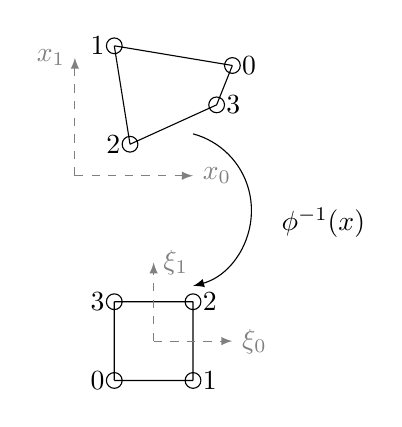
\begin{tikzpicture}{scale=2.0}
          
          \draw (0,0) circle[radius=.1] node[left]{0}-- 
          (1,0) circle[radius=.1] node[right]{1} -- 
          (1,1) circle[radius=.1] node[right]{2} -- 
          (0,1) circle[radius=.1] node[left]{3} -- (0,0);
          \draw[color=gray, dashed, -latex] (0.5,0.5) -- (1.5,0.5) node[right]{$\xi_0$};
          \draw[color=gray, dashed, -latex] (0.5,0.5) -- (0.5,1.5) node[right]{$\xi_1$};
          
          \draw (.2,3) circle[radius=.1] node[left]{2}
          -- (1.3,3.5) circle[radius=.1] node[right]{3}
          -- (1.5,4) circle[radius=.1] node[right]{0}
          -- (0,4.25) circle[radius=.1] node[left]{1}
          -- (.2,3);
          \draw[color=gray,dashed, -latex] (-0.5, 2.6) -- (1, 2.6) node[right]{$x_0$};
          \draw[color=gray,dashed, -latex] (-0.5, 2.6) -- (-0.5, 4.1) node[left]{$x_1$};
          
          \draw[latex-] (1,1.2) arc (-75:75:1);
          \draw (2,2) node[right]{$\phi^{-1}(\tensor{x})$};
          
        \end{tikzpicture}
      \end{figure}
    \end{column}
  \end{columns}

\end{frame}


%==============================================================
\begin{frame}{Change of integration bounds}

  \begin{columns}
    \begin{column}{0.5\textwidth}
      \begin{itemize}
      \item
        The transformation results in:
        \begin{align*}
          \int_{\Omega_e}\nabla v \cdot &\nabla u \dV = \\
          &\int_{\Omega_0}\nabla v \cdot \nabla u \;\mathrm{det}(\tensor{J})\dV_0 \\
          %
          %
          \\
          \text{Where } &\tensor{J} = \frac{\partial \tensor{\phi}}{\partial \tensor{\xi}} > 0
        \end{align*}
      \end{itemize}
    \end{column}
    \begin{column}{0.5\textwidth}
      \begin{figure}
        \centering
        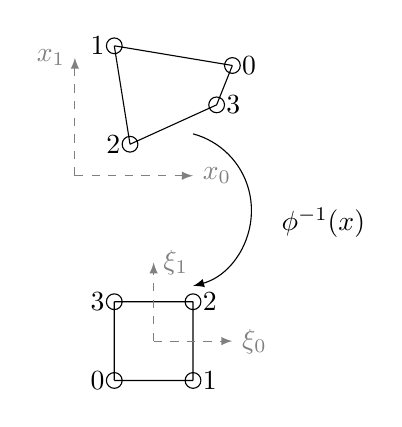
\begin{tikzpicture}{scale=2.0}
          
          \draw (0,0) circle[radius=.1] node[left]{0}-- 
          (1,0) circle[radius=.1] node[right]{1} -- 
          (1,1) circle[radius=.1] node[right]{2} -- 
          (0,1) circle[radius=.1] node[left]{3} -- (0,0);
          \draw[color=gray, dashed, -latex] (0.5,0.5) -- (1.5,0.5) node[right]{$\xi_0$};
          \draw[color=gray, dashed, -latex] (0.5,0.5) -- (0.5,1.5) node[right]{$\xi_1$};
          
          \draw (.2,3) circle[radius=.1] node[left]{2}
          -- (1.3,3.5) circle[radius=.1] node[right]{3}
          -- (1.5,4) circle[radius=.1] node[right]{0}
          -- (0,4.25) circle[radius=.1] node[left]{1}
          -- (.2,3);
          \draw[color=gray,dashed, -latex] (-0.5, 2.6) -- (1, 2.6) node[right]{$x_0$};
          \draw[color=gray,dashed, -latex] (-0.5, 2.6) -- (-0.5, 4.1) node[left]{$x_1$};
          
          \draw[latex-] (1,1.2) arc (-75:75:1);
          \draw (2,2) node[right]{$\phi^{-1}(\tensor{x})$};
          
        \end{tikzpicture}
      \end{figure}
    \end{column}
  \end{columns}

\end{frame}


%==============================================================
\subsection{Intra-element Interpolation}
%==============================================================
\begin{frame}{Interpolation}

  \begin{itemize}
  \item
    We can interpolate within an element using nodal values
    and nodal ``shape functions''
  \item
    Shape functions satisfy ``partition of unity'', the ``kronecker delta'' property,
    and have compact support on $\Omega$
    \begin{align*}
      \sum_{A=1}^{elem\_nodes} N^A(\tensor{\xi}) &= 1 \\
      N^A(\tensor{\xi}^B) = &\left\{
      \begin{array}{c}
        1 \;\; A=B\\
        0 \;\; A\neq B
      \end{array}\right. \\
    \end{align*}
  \item
    Fields defined on a node ($u^A$) can be interpolated inside an element by
    \begin{align*}
      u(\xi) &= \sum_A N^A(\xi) u^A & \tensor{x}(\xi) = \sum_A N^A(\xi) \tensor{x}^A
    \end{align*}
  \end{itemize}

\end{frame}


%==============================================================
\subsection{Numerical Integration}
%==============================================================
\begin{frame}{Numerical Integration}
  \begin{itemize}
  \item
    For trivial cases, the integrals involved in FEM can be evaluated analytically
  \item
    In general, this is not possible  $\implies$ Gaussian Quadrature
    \begin{align*}
    \int_{\Omega} f(x) \dV \approx \sum_{x_i \in \{QP\}} f(x_i)\cdot w_i
    \end{align*}
  \item
    Quadrature points $x_i \in \{QP\}$ and weights $w_i$ chosen
    to approximate integral to specified order of accuracy
  \end{itemize}
\end{frame}

%==============================================================
\begin{frame}{Gaussian Quadrature}

  \begin{columns}
    \begin{column}{0.5\textwidth}
      \begin{itemize}
      \item
        Quadrature rules defined on parent element
      \item
        Typically use Gauss-Legendre quadrature (see wikipedia)
      \item
        Quadrature rules can be computed to calculate any order
        polynomial exactly
      \item
        Not useful to integrate more accurately than you interpolate
      \end{itemize}
    \end{column}
    \begin{column}{0.5\textwidth}
      \begin{figure}
        \centering
        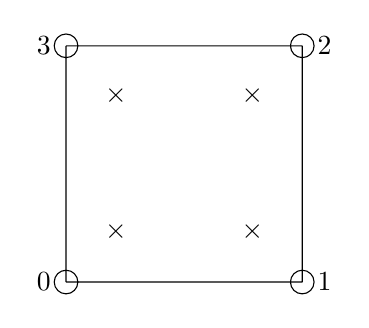
\begin{tikzpicture}[scale=1.5]

          \draw (-1,-1) circle[radius=.1] node[left=2pt]{0}-- 
          (1,-1) circle[radius=.1] node[right=2pt]{1} -- 
          (1,1) circle[radius=.1] node[right=2pt]{2} -- 
          (-1,1) circle[radius=.1] node[left=2pt]{3} -- (-1,-1);

          \draw (-.577,-.577) node{$\times$};
          \draw (.577,-.577) node{$\times$};
          \draw (.577,.577) node{$\times$};
          \draw (-.577,.577) node{$\times$};


        \end{tikzpicture}
        \caption{
          Two-point (per dimension) quadrature over the canonical
          quadrilateral element.
        }
      \end{figure}
    \end{column}
  \end{columns}
  
\end{frame}


%==============================================================
\subsection{Putting it all together}
%==============================================================
\begin{frame}{Making it look like code}
  \begin{itemize}
  \item
    The weak form of PDEs can be (with a little practice) written
    almost directly into code
  \item
    The goal is to write the integrals in a matrix-vector form
    \begin{align*}
      \int_{\Omega_0} \nabla v \cdot \nabla u \mathrm{det}\tensor{J}\dV_0 &\approx
      \int_{\Omega_0} \left(\sum_A \frac{\partial N^A}{\partial \tensor{x}} v^A\right) 
      \cdot \left(\sum_B \frac{\partial N^B}{\partial \tensor{x}} u^B\right) 
      \mathrm{det}\tensor{J}\dV_0
    \end{align*}
  \item
    Exploit linearity:
    \begin{align*}
      (v^A)^T\left(\sum_A \sum_B \int_{\Omega_0} \frac{\partial N^A}{\partial \tensor{x}} 
      \cdot \frac{\partial N^B}{\partial \tensor{x}}
      \mathrm{det}\tensor{J}\dV_0 \right) (u^B)
      &= \vec{v}^T \tensor{K}_e \,\vec{u}_e
    \end{align*}
  \end{itemize}
\end{frame}


%==============================================================
\begin{frame}{Finishing it off}
  \begin{itemize}
  \item
    The previous expression produces a local $\tensor{K}_e \in \mathbb{R}^{Npe\times Npe}$ (stiffness) matrix
  \item
    These matrices must be ``added'' together via assembly into a global linear system
  \item
    Boundary conditions can be either added at the element level or at the global
    linear system level
  \item
    Flux boundary conditions (given by surface integral ignored since beginning)
    must also be integrated (via quadrature over faces comprising $\partial \Omega_N$)
  \end{itemize}
\end{frame}
